% --
% machine learning

\section{Neural Networks for KWS}
\sectionheader{Neural Networks for KWS}

\begin{frame}
  \frametitle{Fully Connected Layer}
  \begin{figure} 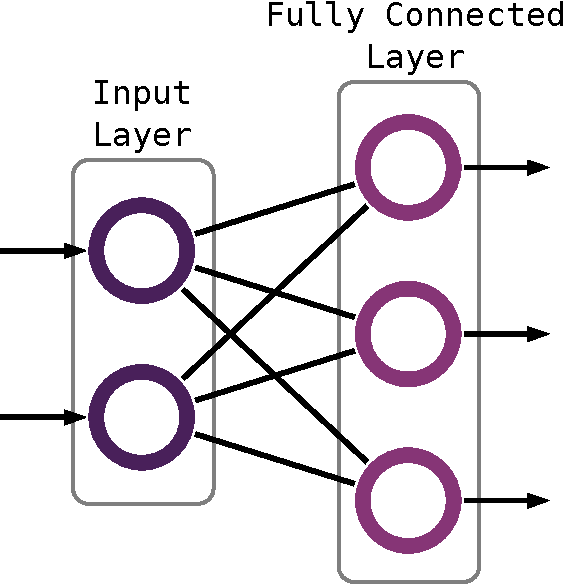
\includegraphics[width=0.5\textwidth]{../4_nn/figs/nn_theory_fc.pdf} \end{figure}
\end{frame}

\begin{frame}
  \frametitle{Convolutional Neural Networks}
  \begin{figure} 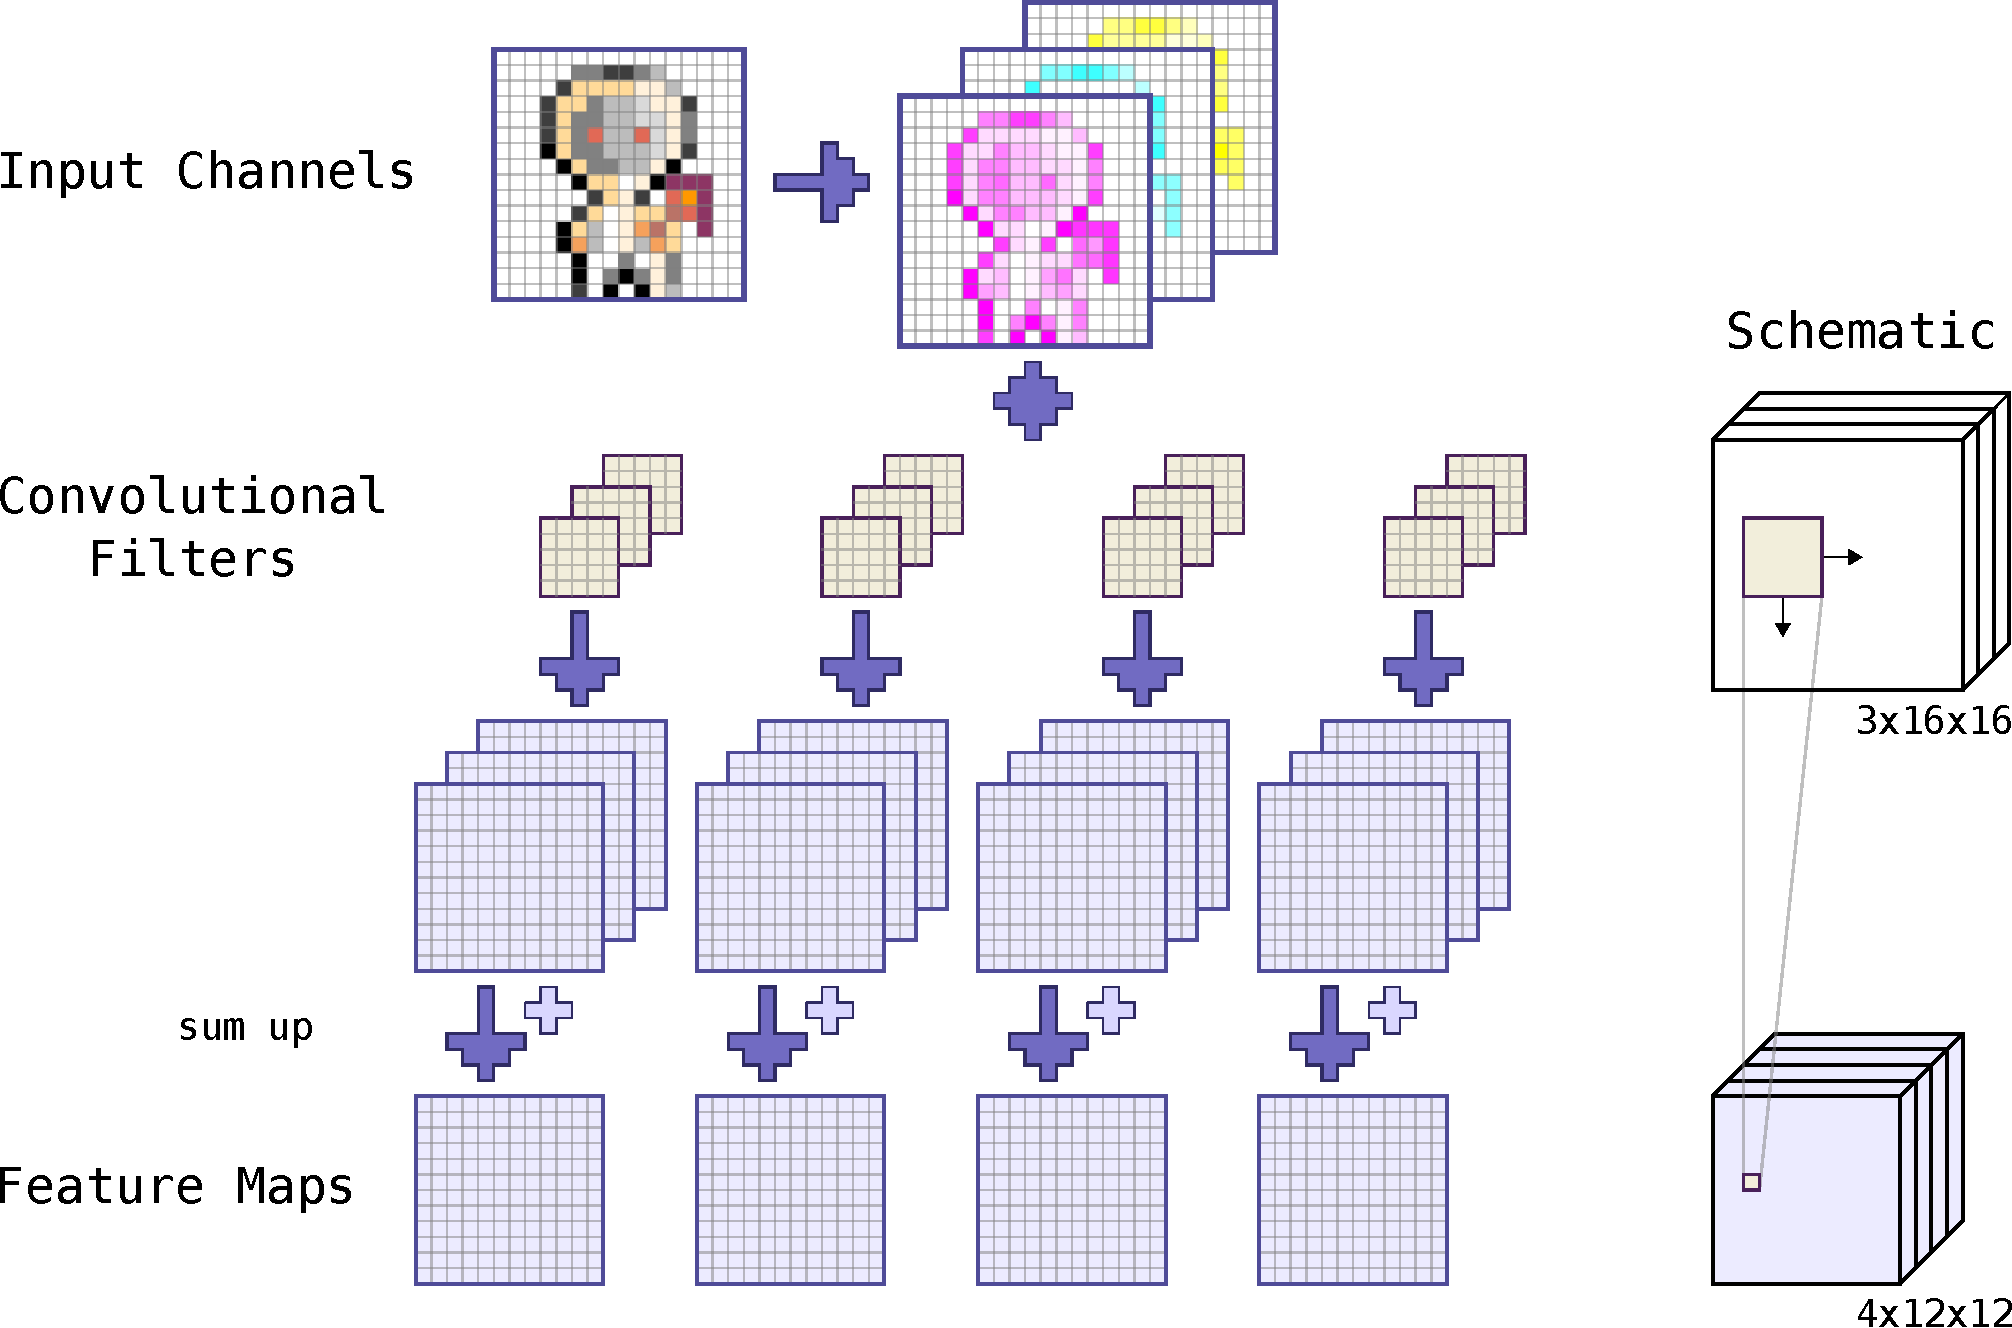
\includegraphics[width=0.8\textwidth]{../4_nn/figs/nn_theory_cnn_basics.pdf} \end{figure}
\end{frame}

\begin{frame}
  \frametitle{Traditional Network (conv-trad)}
  \begin{figure} 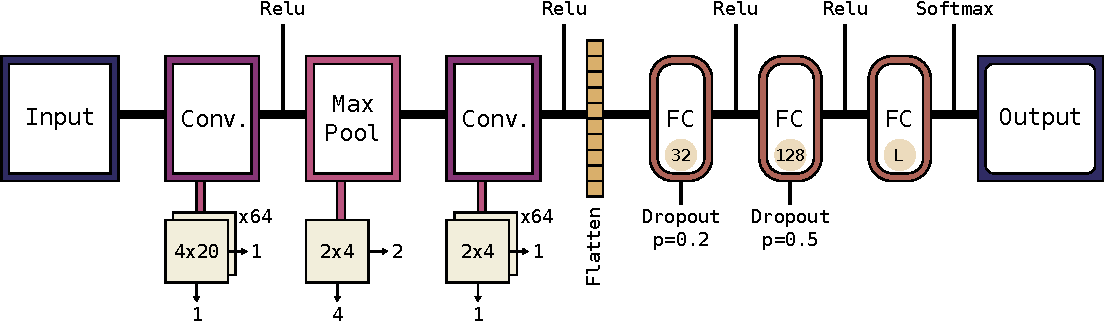
\includegraphics[width=1.0\textwidth]{../4_nn/figs/nn_arch_cnn_trad.pdf} \end{figure}
\end{frame}

\begin{frame}
  \frametitle{Frequency Striding Network (conv-fstride)}
  \begin{figure} 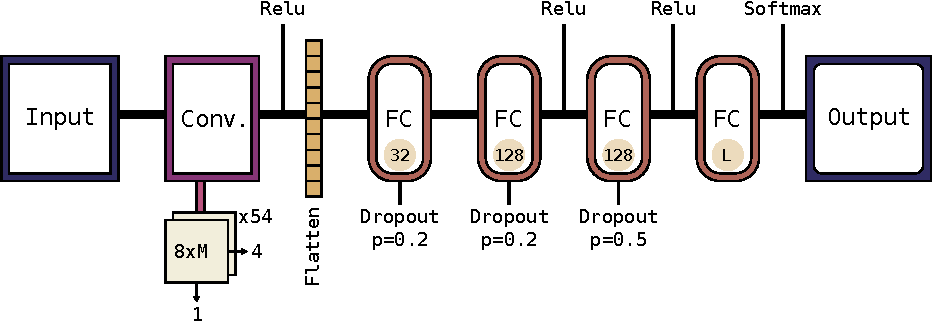
\includegraphics[width=1.0\textwidth]{../4_nn/figs/nn_arch_cnn_fstride.pdf} \end{figure}
\end{frame}

\begin{frame}
  \frametitle{Time Striding Network(conv-jim)}
  \begin{figure} 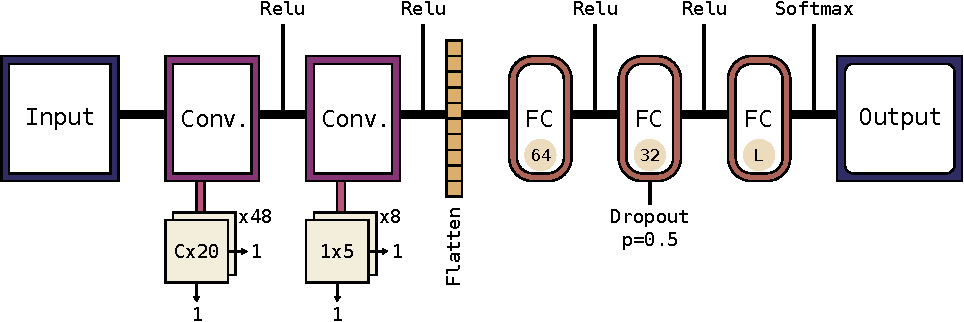
\includegraphics[width=1.0\textwidth]{../4_nn/figs/nn_arch_cnn_jim.pdf} \end{figure}
\end{frame}

